%%%%%%%%%%%%%%%%%%%%%%%%%%%%%%%%%%%%%%%%%%%%%%%%%%%%%%%%%%%%%%%%%%%%%%%%%%%%%%%%
% Template for USENIX papers.
%
% History:
%
% - TEMPLATE for Usenix papers, specifically to meet requirements of
%   USENIX '05. originally a template for producing IEEE-format
%   articles using LaTeX. written by Matthew Ward, CS Department,
%   Worcester Polytechnic Institute. adapted by David Beazley for his
%   excellent SWIG paper in Proceedings, Tcl 96. turned into a
%   smartass generic template by De Clarke, with thanks to both the
%   above pioneers. Use at your own risk. Complaints to /dev/null.
%   Make it two column with no page numbering, default is 10 point.
%
% - Munged by Fred Douglis <douglis@research.att.com> 10/97 to
%   separate the .sty file from the LaTeX source template, so that
%   people can more easily include the .sty file into an existing
%   document. Also changed to more closely follow the style guidelines
%   as represented by the Word sample file.
%
% - Note that since 2010, USENIX does not require endnotes. If you
%   want foot of page notes, don't include the endnotes package in the
%   usepackage command, below.
% - This version uses the latex2e styles, not the very ancient 2.09
%   stuff.
%
% - Updated July 2018: Text block size changed from 6.5" to 7"
%
% - Updated Dec 2018 for ATC'19:
%
%   * Revised text to pass HotCRP's auto-formatting check, with
%     hotcrp.settings.submission_form.body_font_size=10pt, and
%     hotcrp.settings.submission_form.line_height=12pt
%
%   * Switched from \endnote-s to \footnote-s to match Usenix's policy.
%
%   * \section* => \begin{abstract} ... \end{abstract}
%
%   * Make template self-contained in terms of bibtex entires, to allow
%     this file to be compiled. (And changing refs style to 'plain'.)
%
%   * Make template self-contained in terms of figures, to
%     allow this file to be compiled. 
%
%   * Added packages for hyperref, embedding fonts, and improving
%     appearance.
%   
%   * Removed outdated text.
%
%%%%%%%%%%%%%%%%%%%%%%%%%%%%%%%%%%%%%%%%%%%%%%%%%%%%%%%%%%%%%%%%%%%%%%%%%%%%%%%%

\documentclass[letterpaper,twocolumn,10pt]{article}
\usepackage{usenix2019_v3}

% to be able to draw some self-contained figs
\usepackage{tikz}
\usepackage{amsmath}

% inlined bib file
\usepackage{filecontents}

\usepackage{graphicx}
\graphicspath{{./}}

%-------------------------------------------------------------------------------
\begin{filecontents}{\jobname.bib}
%-------------------------------------------------------------------------------


@article{braineeg,
  title={Predicting Age From Brain EEG Signals—A Machine Learning Approach},
  author={Obada Al Zoub, Chung Ki Wong, Rayus Tiberius Kuplicki},
  year={2018},
  publisher={https://www.frontiersin.org/}
}

@article{braineeg2,
  title={Methods of EEG Signal Features Extraction Using Linear Analysis in Frequency and Time-Frequency Domains},
  author={Amjed S. Al-Fahoum and Ausilah A. Al-Fraihat},
  year={2014},
  publisher={Hindawi Publishing Corporation, ISRN Neuroscience}
}

@article{kaggle_link,
  title={Methods of EEG Signal Features Extraction Using Linear Analysis in Frequency and Time-Frequency Domains},
  author={Amjed S. Al-Fahoum and Ausilah A. Al-Fraihat},
  year={2014},
  publisher={Hindawi Publishing Corporation, ISRN Neuroscience}
}


\end{filecontents}

%-------------------------------------------------------------------------------
\begin{document}
%-------------------------------------------------------------------------------

%don't want date printed
\date{}

% make title bold and 14 pt font (Latex default is non-bold, 16 pt)
\title{\Large \bf Age Prediction from EEG signals using Spark MLLib}

%for single author (just remove % characters)
\author{
{\rm Emmanouil Anagnostakis}\\
Computer Science Department, University of Crete
\and
{\rm Konstantinos Spiridakis}\\
Computer Science Department, University of Crete
% copy the following lines to add more authors
% \and
% {\rm Name}\\
%Name Institution
} % end author

\maketitle

%-------------------------------------------------------------------------------
\begin{abstract}
%-------------------------------------------------------------------------------
In this study, we seek to find a strong binding between EEG signals and Machine Learning(ML).Our motivation is to understand the correlation between signals and the gravity of each one.In this way, we are able to identify patterns on EEG signals to make predictions about the real patient’s age.We tested various prediction models and we are going to  present those which achieved higher scores.This is a research with high potential to improve ,while many parameters can be readjusted and more models can be tested, given more time and computing power.We believe that our work assembles another big step on connecting large datasets of EEG signals and Machine Learning.

\end{abstract}

%-------------------------------------------------------------------------------
\section{Introduction}
%-------------------------------------------------------------------------------
For many years the human brain has been studied in various ways. This work focuses on a metric called BrainAGE, which is the distance in years between the predicted age and real age. Majority of studies similar to this, aim to compare BrainAGE between healthy and unhealthy patients.
However, this work will provide you with models on just predicting BrainAGE and ways to optimize it.
\par
In particular,  BrainAGE prediction is based on EEG signals in this case.According to older studies, EEG features(values) and their correlation can project on an age function which changes based on these values.The electroencephalogram is a recording of electrical activity of the brain from the scalp.From the recorded waveforms we extract signal intensity and frequency.Frequencies are divided in categories accordingly to their value (Delta,Theta,Alpha,Beta).However, categories min-max values will eventually play a key role on prediction models.
The dataset is retrieved from the publicly available Temple University EEG Corpus, specifically it is a part of the “TUH Abnormal EEG Corpus”.It is also available on \href{https://www.kaggle.com/ayurgo/data-eeg-age-v1}{Kaggle}.  The primal purpose of the original dataset is to distinguish between normal and abnormal EEG signals. We, however, are interested in studying normal EEG alone. The data contains 1297 patient’s recordings of slightly various length comparing with similar older study from Dimitriadis and Salis(2017),where authors used functional connectivity features from EEG to predict age from 94 healthy subjects. 
There are two folders: train (1171 files) and eval (126 files) cumulatively ~100GB of raw text. In each folder there are .csv files where their first row contains the age, the second row contains the EEG channels’ names used in the recording  and the signal data follows from the third row.

\begin{figure}[h!]
  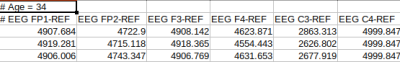
\includegraphics[width=0.5\textwidth]{ds_lines}
\caption{Three rows from the dataset.}
\end{figure}

EEG signals are presented as float numbers. Each column represents a different signal, therefore a different position of electrodes placed on human brain. 
e.g. FP1: front lobe of the cerebrum
\par
In this study, we proposed methods to predict BrainAGE using different features of EEG signals. First, we reduced the data where we applied normalization in order to fit on models.Then, we applied a set of machine learning (ML) methods to predict age from features. Finally, after multiple validations and tests we selected the best of three prediction models based on metrics RMSE and MAE. The overall results show that there is much space for improvement.



%-------------------------------------------------------------------------------
\section{Design}
In this section we describe the preparation and the methods of our approach.Data preparation or pre-processing is a major step before testing prediction models.Features reduction is basically ,selecting best features for input.Keeping out the “abnormal” cells improvises results and makes conclusions more reliable.

\subsection{Data Preprossesing}
%-----------------------------------

Each file in the train and eval dataset , cleaned by a mechanism that checked for whole columns with empty cells and removed them.Observing the dataset ,it was clear that not all patients had the same number of features.So predicting features that do not exist would cause additional problems, extravagant features were removed.Another pre-processing step was the elimination of columns with zero feature dispersion.We calculated the average of each “suspect” column and eliminate those whose values had very small difference from the average.Another major role change was dataset balancing .Constructing a prediction model with uneven age percentages equals on puting heaviest weights on specific ages.For example,if age 44 had +100 examinations (rows of features) from each other age , then age 44 will be predicted more often.Constructing models with same amount of examinations from each age fixes dataset imbalance.Last but not least,scaling and normalizing training data was a good idea because of features’ range.Unfortunately, it didn’t provide much of improvement in any model.

\subsection{Models}

In the remainder of this section we will briefly describe the three models that were selected to be used on a large data scale to perform on AWS clusters. We also tried more models which will be analyzed below in the evaluation section and chose the three best for calculating our results shown in figures 1 and 2.

\begin{figure}[h!]
  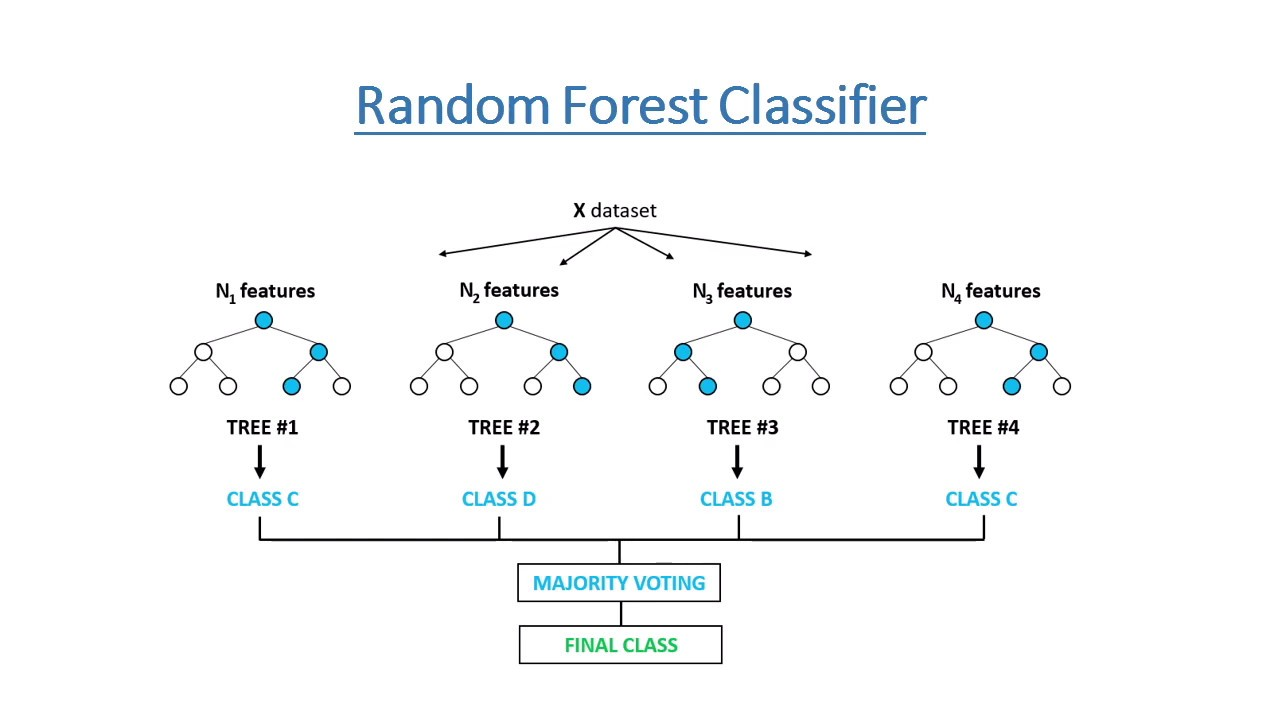
\includegraphics[width=0.5\textwidth]{random_forest_figure}
\caption{Example of how a Random Forest Classification looks like.}
\end{figure}

\subsection{Random Forest Classification}
%-----------------------------------

Random forest (see Figure 1), like its name implies, consists of a large number of individual decision trees that operate as an ensemble.
Each individual tree in the random forest spits out a class prediction and the class with the most votes becomes our model’s prediction.
The fundamental concept behind random forest is a simple but powerful one — the wisdom of crowds. The low correlation between models is the key. 
Just like how investments with low correlations (like stocks and bonds) come together to form a portfolio that is greater than the sum of its parts, uncorrelated models can produce ensemble predictions that are more accurate than any of the individual predictions.
The reason for this wonderful effect is that the trees protect each other from their individual errors (as long as they don’t constantly all err in the same direction). 
While some trees may be wrong, many other trees will be right, so as a group the trees are able to move in the correct direction. So the prerequisites for random forest to perform well are:
There needs to be some actual signal in our features so that models built using those features do better than random guessing.
The predictions (and therefore the errors) made by the individual trees need to have low correlations with each other.

\begin{figure}[h!]
  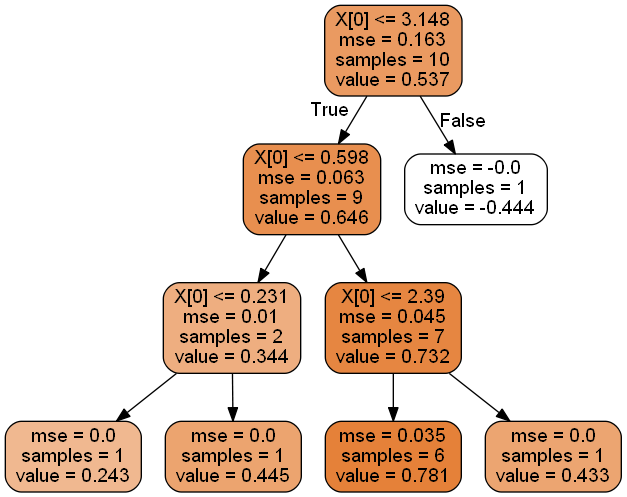
\includegraphics[width=0.5\textwidth]{decision_tree_regression}
\caption{Example of a Decision Tree Regression.}
\end{figure}

\subsection{Decision Tree Regression}
%-----------------------------------

A decision tree (see Figure 2) is arriving at an estimate by asking a series of questions to the data, each question narrowing our possible values until the model get confident enough to make a single prediction. 
The order of the question as well as their content are being determined by the model. In addition, the questions asked  are all in a True/False form.
The decision of making strategic splits heavily affects a tree’s accuracy. The decision criteria is different for classification and regression trees.
Decision trees regression normally use mean squared error (MSE) to decide to split a node in two or more sub-nodes. Suppose we are doing a binary tree the algorithm first will pick a value, and split the data into two subset. For each subset, it will calculate the MSE separately. 
The tree chooses the value with results in smallest MSE value.

\begin{figure}[h!]
  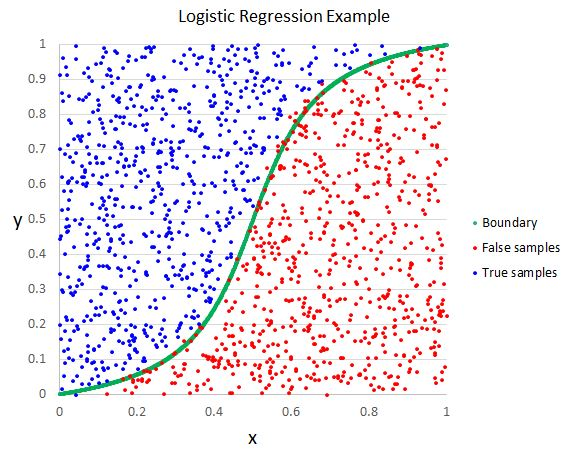
\includegraphics[width=0.5\textwidth]{logistic_regression_example}
\caption{An example of how Logistic Regression does decide false and true samples.}
\end{figure}

\subsection{Logistic Regression}
%-----------------------------------

Logistic regression (see Figure 3) is a statistical model that in its basic form uses a logistic function to model a binary dependent variable, although many more complex extensions exist. In regression analysis, logistic regression (or logit regression) is estimating the parameters of a logistic model (a form of binary regression).
 
Types of Logistic Regression are:
1. Binary Logistic Regression:
The categorical response has only two 2 possible outcomes. Example: Spam or Not
2. Multinomial Logistic Regression:
Three or more categories without ordering. Example: Predicting which food is preferred more (Veg, Non-Veg, Vegan)
3. Ordinal Logistic Regression:
Three or more categories with ordering. Example: Movie rating from 1 to 5
In our example we adopt the ordinal logistic regression technique.

%-------------------------------------------------------------------------------
\section{Evaluation}
%-------------------------------------------------------------------------------

We tried a variety of different models to understand which technique would better suit our problem. The models were taken from both categories, Classification and Regression. Despite our dataset having continuous features and presenting itself like a regression problem, classification algorithms were less affected by overfitting and provided more concrete predictions for the age.
\par The models that will be evaluated are the following: Decision Tree Classification, Decision Tree Regression, Random Forest Classification, Random Forest Regression, Gradient Boosted Tree Regression, Logistic Regression, Factorization Machines Regression and Linear Regression. We also tried to implement Survival Regression, KNN and K-means clustering without success. Various feature transformers were used described in section 2. Cross validation using grid search was implemented in order to find the best model parameters. Below follows the evaluation structured in categories regarding each selected and rejected models and providing descriptions on two figures showing the RMSE and MAE performance of each of the selected models respectively. 


\begin{figure}[h!]
  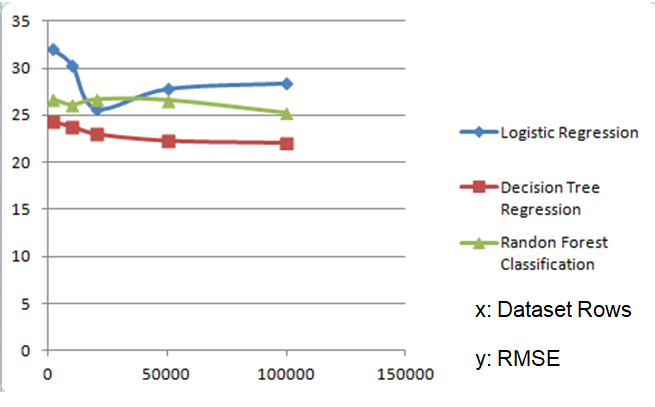
\includegraphics[width=0.5\textwidth]{grafima_rmse}
\caption{Root Mean Squared Error of each selected model per number of rows of each dataset file.}
\end{figure}

\begin{figure}[h!]
  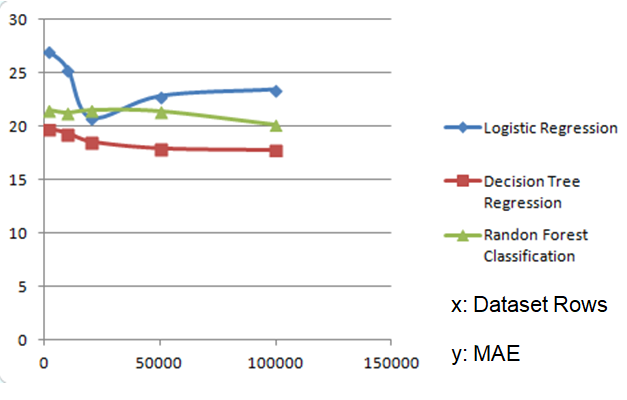
\includegraphics[width=0.5\textwidth]{grafima_mae}
\caption{Mean Average Error of each selected model per number of rows of each dataset file.}
\end{figure}

\begin{figure}[h!]
  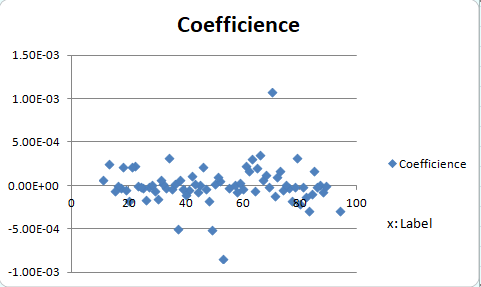
\includegraphics[width=0.5\textwidth]{coefficience}
\caption{Coefficience of Logistic Regression per label.}
\end{figure}

\subsection{Hardware and Software}

We worked both locally with small experiments and on AWS clusters with larger parts of the dataset. Our local computers have 16 gb of ram and a 3.2 ghz intel processor each. This means we could test up to a total of 6\% of the dataset locally divided by 2 which means each person could run a 3\% of the dataset on their computer. The total dataset size is 100g so each person used 3g locally. Then by creating an AWS cluster of 1 master and 1 slave m5-2xlarge instance of 32 gb memory and 8 processors (64gb total memory and 16 processors) we were able to scale to 30\% of the dataset which equals to 30g of data. The data were partitioned in 16 pieces at load and then when we parallelized our data structures we used 50 partitions. We used one AWS account to not waste time on setting up the second account and ran for 12 hours consuming 11.11 dollars using spot billing which was enough to create our results as we finished all development locally and we just needed to use a larger part of the dataset. Each person ran their own experiments with 30g of data which means that the project needs were fulfilled.


\subsection{Selected Models}

	We tested all the machine learning models listed in the introduction of the evaluation section and decided to move to the cluster with the three models shown in figure 1 and 2. The models were evaluated using two common techniques, the RMSE (Root Mean Squared Error) and the MAE (Mean Average Error). The RMSE represents the square root of the second sample moment of the differences between predicted values and observed values or the quadratic mean of these differences. MAE measures the average magnitude of the errors in a set of predictions, without considering their direction. It's the average over the test sample of the absolute differences between prediction and actual observation where all individual differences have equal weight.
\par	Let’s start by describing the evaluation of the Random Forest Classification model. We tried to use and test all the hyperparameters starting from maxBins, maximum number of bins used for discretizing continuous features and for choosing how to split on features at each node. The more the bins the higher the granularity. After testing several values with CrossValidation and manually we decided that the default value of 32 produced the best results. We then tried to variate the maximum depth of each tree, with the maxDepth variable. We came to a conslusion to chose the default of 5. The next hyperparameter checked is the minInstancesPerNode, minimum number of instances each child must have after split. If a split causes the left or right child to have fewer than minInstancesPerNode, the split will be discarded as invalid. Again after several tries the default value of 1 was picked. The third hyperparameter is the minWeightFractionPerNode, minimum fraction of the weighted sample count that each child must have after split. If a split causes the fraction of the total weight in the left or right child to be less than minWeightFractionPerNode, the split will be discarded as invalid. The default value of 0.0 was picked. We also tested changing the minInfoGain, minimum information gain for a split to be considered at a tree node. Once again the default value of 0.0 was picked. The last parameter is the numTrees, number of decision trees used. We also went with the default using the value of 20. Now let’s analyze the performance on figure 1 showing the RMSE per feature lines of each dataset file. The RMSE is not showing much of an improvement as the number of features fed to the model are increasing, starting from a point of 26.00 with 2000 per file and decreasing to 25.00 with 100000 lines per file. Figure 2 shows MAE per lines of features per file. Once again the improvement is not of significance as it starts at 21.00 with 2000 lines and decreases to 20.00 with 100000 lines.
\par	Continuing to evaluate the Decision Tree Regression model. We tried to use and test all the hyperparameters as we did with Random Forest starting from maxBins. After testing several values with CrossValidation and manually we decided that the default value of 32 produced the best results like in Random Forest. We tried to variate the maximum depth of the tree, with the maxDepth variable. We chose the value of 30. The next hyperparameter checked is the minInstancesPerNode. After several tries the value of 16 was picked. The third hyperparameter is the minWeightFractionPerNode. The default value of 0.0 was picked. We also tested changing the minInfoGain. Once again the default value of 0.0 was picked. In terms of the performance on figure 1 showing the RMSE per feature lines of each dataset file, RMSE is showing a significant improvement as the number of features fed to the model are increasing, starting from a point of 25.00 with 2000 per file and decreasing to 22.00 with 100000 lines per file. Checking figure 2 we see an analogous improvement starting at 20.00 with 2000 lines and decreasing to 18.00 with 100000 lines.
\par	The last of the selected models to be run at scale is the Logistic Regression. We had three different hyperparameters at our disposal, the maxIter (max iterations run to train the model), regParam (regularization parameter) and elasticNetParam to prevent overfitting. We tried lots of different values for these fields but the ones that seemed to match were 60 iterations, 0.01 for regularization parameter and 0.08 for elastic net. In terms of the performance on figure 1 showing the RMSE per feature lines of each dataset file, RMSE is showing to be unstable by decreasing from 32.00 for 2000 lines to 25.00 for 20000 lines and then going slightly upwards to reach 28 for 100000 lines per file. Checking figure 2 we see an analogous improvement starting at 27.00 with 2000 lines and decreasing to 21.00 with 20000 lines and then going up to 23.00 for 100000 lines.




\subsection{Rejected Models}

	We rejected many models like the Decision Tree Classifier, the Random Forest Regression,  Factorization machines Regression, the Gradient Boosted Tree Regressor and the Linear Regressor. Every single one of them was more or less overfitting on certain values and that effect could not be undone even if we had options of hyperparameters to change or were in lack of them. The Random forest, Decision tree and Gradient Boosted approaches offered the same hyperparameters described above in section 3.2 for their counterparts but even after a lot of tries and cross validation we couldn’t find a set of them to give a satisfying error or prevent overfitting. Same thing happened with trying to change iterations, regularization parameter and elastic net on Linear Regression but the overfitting there was worse. We suspect that we needed to take a different path on feature extraction and transformation to get rid of it. We also tried to implement Survival Regression but it needed a censor value in the Labeled Points to work and we put it aside. Finally we didn’t find enough information and resources for a successful KNN or K-means clustering algorithm implementation.


%-------------------------------------------------------------------------------
\section{Conclusion}
%-------------------------------------------------------------------------------

We presented a machine learning approach to a medical problem regarding encephalography. We downloaded a dataset of raw EEG signals provided in the Kaggle website which included the age of the patients. Afterwards we used Spark to process the given data and create suitable RDDs and data structures containg the age as the label and the EEG signals as the features to be fed to ML models provided by the MLLib library of Spark. The evaluation of the models was done by extracting the RMSE (Root Mean Squared Error) and the MAE (Mean Average Error) of each model. The work shows that it is possible for age to be extracted by EEG signals which is also shown by relative work from the papers (Predicting Age From Brain EEG Signals—A Machine Learning Approach) \cite{braineeg} and (Methods of EEG Signal Features Extraction Using Linear Analysis in Frequency and Time-Frequency Domains) \cite{braineeg2} . The models that perform better are the Decision Tree Regressor, the Random Forest Classifier and the Logistic Regression. The other models were basically rejected because of overfitting. There is a huge room for improvement judging by the results and that can be a very promising field for further research.


%-------------------------------------------------------------------------------
\bibliographystyle{plain}
\bibliography{\jobname}

%%%%%%%%%%%%%%%%%%%%%%%%%%%%%%%%%%%%%%%%%%%%%%%%%%%%%%%%%%%%%%%%%%%%%%%%%%%%%%%%
\end{document}
%%%%%%%%%%%%%%%%%%%%%%%%%%%%%%%%%%%%%%%%%%%%%%%%%%%%%%%%%%%%%%%%%%%%%%%%%%%%%%%%

%%  LocalWords:  endnotes includegraphics fread ptr nobj noindent
%%  LocalWords:  pdflatex acks